\documentclass{article}

\usepackage[utf8]{inputenc}
\usepackage{tikz}
\usetikzlibrary{positioning}
\usepackage{titling}
\usepackage{fancyhdr}

\author{Albina Oscherowa \\ Karsten Lehmann}
\date{06.12.2020}
\title{Programmieren I: Aufgabenblatt 4}

\pagestyle{fancy}
\fancyhf{}
\lhead{\thetitle}
\rhead{\theauthor}
\lfoot{\thedate}
\rfoot{Seite \thepage}

\begin{document}
\section*{Aufgabe 9}

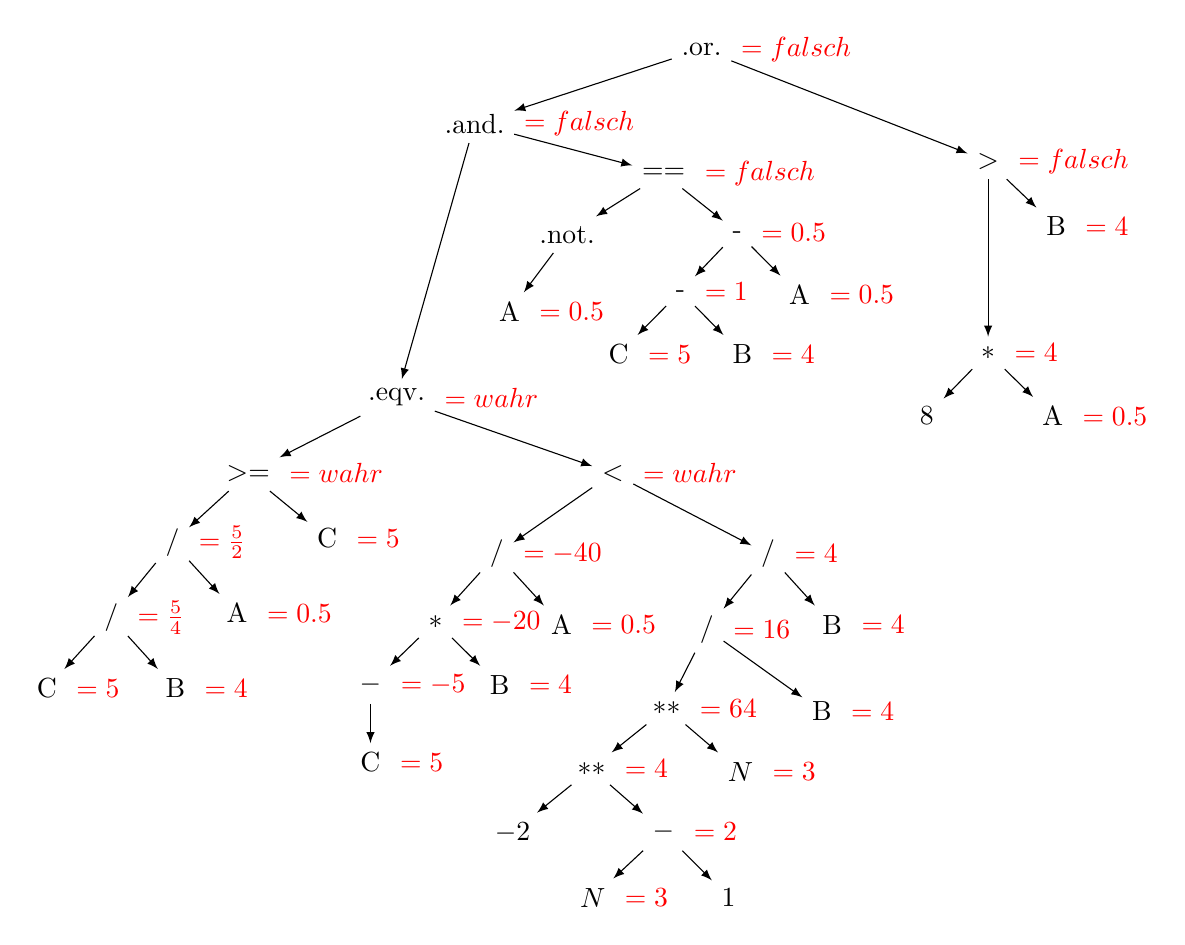
\begin{tikzpicture}
  \node (a) at (0,0) {.or.};
  \node[below right = 1cm and 3cm of a] (aa) {$>$};
  \node[below right = .5cm of aa] (aaa) {B};
  \node[below = 2cm of aa] (aab) {$*$};
  \node[below left = .5cm of aab] (aaba){$8$};
  \node[below right = .5cm of aab] (aabb) {A};

  \node[below left = .5cm and 2cm of a] (ab) {.and.};
  \node[below right = .2cm and 1.5cm  of ab] (aba) {==};  
  \node[below right = .5cm of aba] (abaa) {-}; 
  \node[below right = .5cm of abaa] (abaaa) {A};  
  \node[below left = .5cm of abaa] (abaab) {-};
  \node[below left = .5cm of abaab] (abaaba) {C};
  \node[below right = .5cmof abaab] (abaabb) {B};

  \node[below left = .5cm of aba] (abab) {.not.}; 
  \node[below left = .5cm and 0cm of abab] (ababa) {A}; 

  \node[below left = 3cm and 0cm of ab] (abb) {.eqv.};
  \node[below right = .5cm and 2cm of abb] (abba) {$<$};
  \node[below right = .5cm and 1.5cm of abba] (abbaa) {$/$};
  \node[below right = .5cm of abbaa] (abbaaa) {B};
  \node[below left = .5cm of abbaa] (abbaab) {$/$};
  \node[below left = .5cm and 0cm of abbaab] (abbaaba) {$**$};
  \node[below right = .5cm and 1cm of abbaab] (abbaabb) {B};
  \node[below right = .5cm of abbaaba] (abbaabaa) {$N$};
  \node[below left = .5cm of abbaaba] (abbaabab) {$**$};
  \node[below left = .5cm of abbaabab] (abbaababa) {$-2$};
  \node[below right = .5cm of abbaabab] (abbaababb) {$-$};
  \node[below left = .5cm of abbaababb] (abbaababba) {$N$};
  \node[below right = .5cm of abbaababb] (abbaababbb) {$1$};

  \node[below left = .5cm and 1cm of abba] (abbab) {$/$};
  \node[below right = .5cm of abbab] (abbaba) {A};
  \node[below left = .5cm of abbab] (abbabb) {$*$};
  \node[below right = .5cm of abbabb] (abbabba) {B};
  \node[below left = .5cm of abbabb] (abbabbb) {$-$};
  \node[below = .5cm of abbabbb] (abbabbba) {C};

  \node[below left = .5cm and 1cm of abb] (abbb) {$>=$};
  \node[below right = .5cm of abbb] (abbba) {C};
  \node[below left = .5cm of abbb] (abbbb) {$/$};
  \node[below right = .5cm of abbbb] (abbbba) {A};
  \node[below left = .5cm of abbbb] (abbbbb) {$/$};
  \node[below left = .5cm of abbbbb] (abbbbba) {C};
  \node[below right = .5cm of abbbbb] (abbbbbb) {B};

  \node[red,right = 0cm of a] {$=falsch$};
  \node[red,right = 0cm of aaa] {$=4$};
  \node[red,right = 0cm of aabb] {$=0.5$};
  \node[red,right = 0cm of aab] {$=4$};
  \node[red,right = 0cm of aa] {$=falsch$};
  \node[red,right = 0cm of ab] {$=falsch$};
  \node[red,right = 0cm of aba] {$=falsch$};
  \node[red,right = 0cm of abaa] {$=0.5$};
  \node[red,right = 0cm of abaaa] {$=0.5$};
  \node[red,right = 0cm of abaab] {$=1$};
  \node[red,right = 0cm of abaaba] {$=5$};
  \node[red,right = 0cm of abaabb] {$=4$};
  \node[red,right = 0cm of ababa] {$=0.5$};
  \node[red,right = 0cm of abb] {$=wahr$};
  \node[red,right = 0cm of abba] {$=wahr$};
  \node[red,right = 0cm of abbaa] {$=4$};
  \node[red,right = 0cm of abbaaa] {$=4$};
  \node[red,right = 0cm of abbaab] {$=16$};
  \node[red,right = 0cm of abbaabb] {$=4$};
  \node[red,right = 0cm of abbaaba] {$=64$};
  \node[red,right = 0cm of abbaabaa] {$=3$};
  \node[red,right = 0cm of abbaabab] {$=4$};
  \node[red,right = 0cm of abbaababb] {$=2$};
  \node[red,right = 0cm of abbaababba] {$=3$};
  \node[red,right = 0cm of abbab] {$=-40$};
  \node[red,right = 0cm of abbaba] {$=0.5$};
  \node[red,right = 0cm of abbabb] {$=-20$};
  \node[red,right = 0cm of abbb] {$=wahr$};
  \node[red,right = 0cm of abbba] {$=5$};
  \node[red,right = 0cm of abbbb] {$=\frac{5}{2}$};
  \node[red,right = 0cm of abbbba] {$=0.5$};
  \node[red,right = 0cm of abbbbb] {$=\frac{5}{4}$};
  \node[red,right = 0cm of abbbbba] {$=5$};
  \node[red,right = 0cm of abbbbbb] {$=4$};
  \node[red,right = 0cm of abbabba] {$=4$};
  \node[red,right = 0cm of abbabbb] {$=-5$};
  \node[red,right = 0cm of abbabbba] {$=5$};
  
  \draw[-latex] (a) -> (aa);
  \draw[-latex] (aa) -> (aaa);
  \draw[-latex] (aa) -> (aab);
  \draw[-latex] (aab) -> (aaba);
  \draw[-latex] (aab) -> (aabb);

  \draw[-latex] (a) -> (ab);
  \draw[-latex] (ab) -> (aba);
  \draw[-latex] (aba) -> (abaa);
  \draw[-latex] (abaa) -> (abaaa);
  \draw[-latex] (abaa) -> (abaab);
  \draw[-latex] (abaab) -> (abaaba);
  \draw[-latex] (abaab) -> (abaabb);

  \draw[-latex] (aba) -> (abab);
  \draw[-latex] (abab) -> (ababa);

  \draw[-latex] (ab) -> (abb);
  \draw[-latex] (abb) -> (abba);
  \draw[-latex] (abba) -> (abbaa);
  \draw[-latex] (abbaa) -> (abbaaa);
  \draw[-latex] (abbaa) -> (abbaab);
  \draw[-latex] (abbaab) -> (abbaabb);
  \draw[-latex] (abbaab) -> (abbaaba);
  \draw[-latex] (abbaaba) -> (abbaabaa);
  \draw[-latex] (abbaaba) -> (abbaabab);
  \draw[-latex] (abbaabab) -> (abbaababa);
  \draw[-latex] (abbaabab) -> (abbaababb);
  \draw[-latex] (abbaababb) -> (abbaababba);
  \draw[-latex] (abbaababb) -> (abbaababbb);

  \draw[-latex] (abba) -> (abbab);
  \draw[-latex] (abbab) -> (abbaba);
  \draw[-latex] (abbab) -> (abbabb);

  \draw[-latex] (abbabb) -> (abbabba);
  \draw[-latex] (abbabb) -> (abbabbb);
  \draw[-latex] (abbabbb) -> (abbabbba);

  \draw[-latex] (abb) -> (abbb);
  \draw[-latex] (abbb) -> (abbba);
  \draw[-latex] (abbb) -> (abbbb);
  \draw[-latex] (abbbb) -> (abbbba);
  \draw[-latex] (abbbb) -> (abbbbb);
  \draw[-latex] (abbbbb) -> (abbbbba);
  \draw[-latex] (abbbbb) -> (abbbbbb);
\end{tikzpicture}
\end{document} 